%!TEX root = ../main.tex

\section*{Ejercicio 2}
Descargue el archivo \texttt{Datos.txt} de la página del curso. En este encontrará un conjunto de 21 datos. Copie estos datos y calcule el polinomio de ajuste de grado 5
\[
p(x) = c_0 + c_1x + c_2x^2 + c_3x^3 + c_4x^4 + c_5x^5
\]
utilizando los métodos de ecuaciones normales y factorización QR. Compare sus resultados con los valores certificados $c_i = 1$ para $i = 0, 1, \dots, 5$. Encuentre el residual $\|Ac - y\|_2$ en cada caso, así como la diferencia relativa con respecto a los valores certificados. Escriba sus conclusiones.

\begin{solution}
Al usar el método de ecuaciones normales, se obtienen los coeficientes $\overline{c_0} = 0.999999672214$, $\overline{c_1} =1.000000693559 $, $\overline{c_2} = 0.999999742520$, $c_3 = 1.000000034633$, $\overline{c_4}=0.999999998066$ y $\overline{c_5}= 1.000000000038$ y una norma residual de $9.140802371783\times 10^{5}$, ya que los valores certificados son $c_i=1$ para $i=0,1,\ldots, 5$ el error relativo coincide con el error absoluto, de esta manera tenemos que $|\overline{c_0}-c_0|=0.327785240838 \times 10^{-6}$, $|\overline{c_1}-c_1|= 0.693559258246 \times 10^{-6}$, $|\overline{c_2}-c_2|= 0.257479413678 \times 10^{-6}$, $|\overline{c_3}-c_3|= 0.034633125922 \times 10^{-6}$, $|\overline{c_4}-c_4|= 0.001933269655 \times 10^{-6}$ y $|\overline{c_3}-c_3|= 0.000038107517 \times 10^{-6}$, por lo que obtenemos una precisión de al menos 6 cifras decimales en cada coeficiente.

Ahora, si resolvemos el sistema usando factorización QR, nuestros coeficientes ahora son $\hat{c_0}=1.000000001758$, $\hat{c_1}=0.999999996403$, $\hat{c_2}=1.000000001317$, $\hat{c_3}=0.999999999824$, \\ $\hat{c_4}=1.000000000009$, $\hat{c_5}=0.999999999999$, con una norma residual de $9.140802371783\times 10^{5}$ y los errores correspondientes $|\hat{c_0}-c_0|= 0.000019029222\times 10^{-8}$, $|\hat{c_1}-c_1|=0.000972200098 \times 10^{-8}$, $|\hat{c_2}-c_2|= 0.017562828968\times 10^{-8}$, $|\hat{c_3}-c_3|=0.131761268562 \times 10^{-8}$, $|\hat{c_4}-c_4|= 0.359638396840\times 10^{-8}$, y $|\hat{c_5}-c_5|= 0.175833236859\times 10^{-8}$, en este caso obtuvimos una precisión de al menos 8 cifras decimales en cada coeficiente, lo cual quiere decir que éste método resulta mejor para resolver el sistema que las ecuaciones normales, aún así ambos métodos resultan ser muy precisos, pues los errores son despreciables. Al graficar el conjunto de datos y los dos polinomios obtenidos es practicamente imposible notar la diferencia entre ellos. 
\begin{center}
    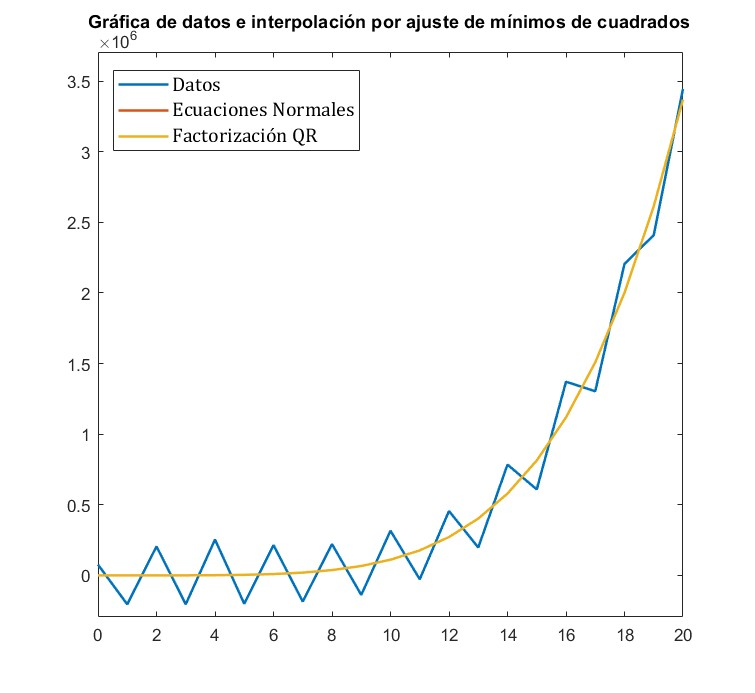
\includegraphics[scale=0.4]{Graficas/Punto2.jpg}
\end{center}
\end{solution}